%%%%%%%%%%%%%%%%%%%%%%%%%%%%%%%%%%%%%%%%%%%%%%%%%%%%%%%%%%%%%%%%%%%%%%%%%%%%%%
%%
%% Dokumentacia k projektu 'Interpret pre jazyk IFJ 2013'
%%
%%
%%%%%%%%%%%%%%%%%%%%%%%%%%%%%%%%%%%%%%%%%%%%%%%%%%%%%%%%%%%%%%%%%%%%%%%%%%%%%%
\documentclass[12pt,a4paper,titlepage,final]{article}

% jazyk
\usepackage[slovak]{babel}
\usepackage[utf8]{inputenc}
% balicky prr odkazy
\usepackage[bookmarksopen,colorlinks,plainpages=false,urlcolor=blue,unicode]{hyperref}
\usepackage{url}
% obrazky
\usepackage[dvipdf]{graphicx}
% velikost stranky
\usepackage[top=3.5cm, left=2.5cm, text={17cm, 24cm}, ignorefoot]{geometry}

\setcounter{secnumdepth}{4}
\usepackage{pdflscape}
\usepackage{afterpage}
\usepackage{capt-of}% or use the larger `caption` package
\usepackage{amsmath}
\usepackage{rotating}
\newcommand{\BigO}[1]{\ensuremath{O\bigl(#1\bigr)}}
\newcommand{\ttlcb}{\texttt{\char 123}}
\newcommand{\ttrcb}{\texttt{\char 125}}
\newcommand{\ttsc}{\texttt{\char 59}}

\begin{document}

%%%%%%%%%%%%%%%%%%%%%%%%%%%%%%%%%%%%%%%%%%%%%%%%%%%%%%%%%%%%%%%%%%%%%%%%%%%%%%
% titulní strana

\def\projname{Dokumentácia IFJ 2013}


\begin{titlepage}

% \vspace*{1cm}
\begin{figure}[!h]
  \centering
  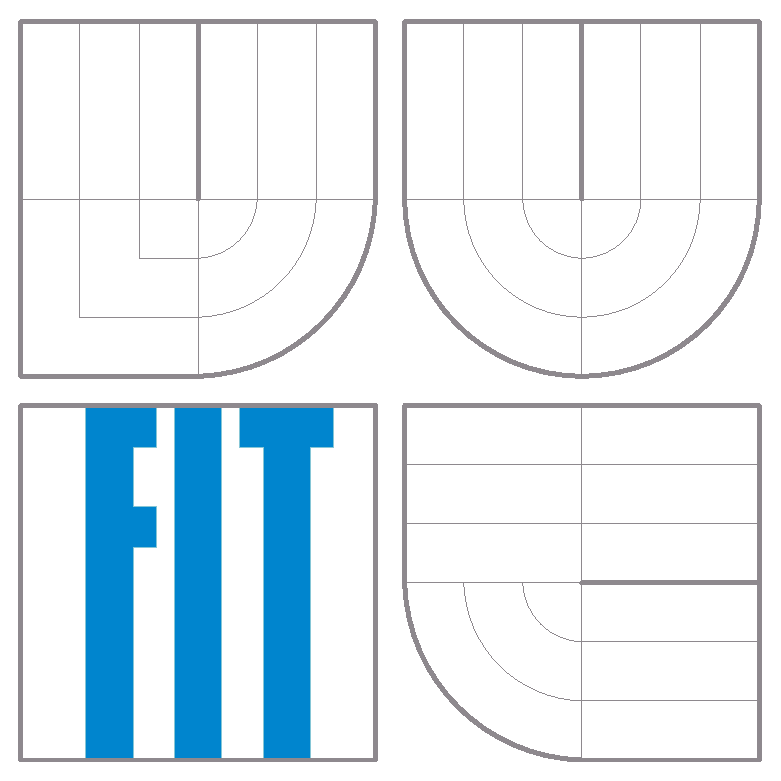
\includegraphics[height=5cm]{doc/img/logo.eps}
\end{figure}
\center Fakulta Informačních Technologií \\
\center Vysoké Učení Technické v Brně \\

\vfill

\begin{center}
\bigskip
\begin{Huge}
\projname\\
\end{Huge}
\begin{large}
Varianta a/4/II\\
{\scriptsize Rozšírenia FOR, FUNEXP, ELSEIF, LOGOP, DEFARG \par}
\end{large}
\end{center}

\vfill

\begin{center}
\begin{Large}
\today
\end{Large}
\end{center}

\vfill

\begin{flushleft}
\begin{large}
Team leader: Marek Milkovič (xmilko01), 20\% \\
Členovia: Lukáš Vrabec (xvrabe07), 20\% \\
\hspace{57px} Ján Spišiak (xspisi03), 20\% \\
\hspace{57px} Ivan Ševčík (xsevci50), 20\% \\
\hspace{57px} Marek Bertovič (xberto00), 20\% \\
\end{large}
\end{flushleft}
\end{titlepage}

%%%%%%%%%%%%%%%%%%%%%%%%%%%%%%%%%%%%%%%%%%%%%%%%%%%%%%%%%%%%%%%%%%%%%%%%%%%%%%
% obsah
\pagestyle{plain}
\pagenumbering{gobble}
\tableofcontents

%%%%%%%%%%%%%%%%%%%%%%%%%%%%%%%%%%%%%%%%%%%%%%%%%%%%%%%%%%%%%%%%%%%%%%%%%%%%%%
% textova zprava
\newpage
\pagestyle{plain}
\pagenumbering{arabic}
\setcounter{page}{1}

%%%%%%%%%%%%%%%%%%%%%%%%%%%%%%%%%%%%%%%%%%%%%%%%%%%%%%%%%%%%%%%%%%%%%%%%%%%%%%

% lex
%%%%%%%%%%%%%%%%%%%%%%%%%%%%%%%%%%%%%%%%%%%%%%%%%%%%%%%%%%%%%%%%%%%%%%%%%%%%%%
\section{Riešenie interpretu} \label{Riesenie interpretu}
%%%%%%%%%%%%%%%%%%%%%%%%%%%%%%%%%%%%%%%%%%%%%%%%%%%%%%%%%%%%%%%%%%%%%%%%%%%%%%

%=============================================================================
\subsection{Lexikálna analýza}
Úlohy lexikálnej analýzy sú:
\begin{enumerate}
    \itemsep0em
    \item čítanie znakov zo vstupu a ich preklad na postupnosť tokenov, ktoré ďalej slúžia syntaktickej analýze
    \item odstránenie komentárov a bielych znakov v zdrojovom programe
    \item nájdenie lexikálnych chýb v zdrojovom programe
\end{enumerate}

Výstup lexikálnej analýzy je zároveň vstupom do syntaktickej analýzy, preto je
lexikálna analýza volaná syntaktickou analýzou. V našom konkrétnom prípade je
výstup lexikálnej analýzy vektor tokenov, kde token je štruktúra obsahujúca
jeho typ (typ je enumerácia všetkých prípustných tokenov)
a v prípade tokenov vyžadujúcich dalšie informácie ako napríklad znakový reťazec,
či prevedenú číselnú hodnotu obsahuje štruktúra aj tieto dáta.
Cieľom je teda prejsť celým súborom až pokým scanner nenájde koniec vstupného súboru
(v C terminológii \texttt{EOF} - End Of File), odhaliť prípadne lexikálne chyby a
v prípade lexikálnej bezchybnosti programu naplniť vektor tokenmi, a pripraviť
tak vstup do syntaktickej analýzy.

Implementácia lexikálnej analýzy spočíva v konštrukcii konečného automatu
(angl. finite state machine), ktorý prečíta znak zo súboru, vyhodnotí
ho a na základe aktuálneho stavu a vstupného znaku môžu nastať tri nasledujúce
možnosti:

1. aktuálny stav neumožnuje pokračovať s daným vstupným znakom a ukončuje tak
jeden token. Prečítaný znak by sa mal navrátiť späť do vstupného súboru, avšak v našej
implementácii sa uloží do pomocnej premennej a nastaví sa príznak, že znak pre
další token bude čítaný nie zo súboru, ale z tejto pomocnej premennej.

2. aktuálny stav umožňuje pokračovať s daným vstupným znakom a nastáva prechod do nového stavu.
V niektorých prípadoch je nový stav totožný s aktuálnym stavom, preto k zmene stavu nedochádza.

3. aktuálny stav neumožnuje pokračovat s daným vstupným znakom a zároveň
nedovoluje ukončiť token. To znamená, že sa v programe nachádza lexikálna chyba.

Špeciálnym prípadom sú stavy pre komentáre a blokové komentáre programu, ktoré
lexikálna analýza registruje, ale kedže sú nepodstatné pre činnosť zdrojového
programu, ignoruje tieto informácie a ďalej ich nespracováva ani neposiela
syntaktickej analýze v podobe tokenu.

Automat lexikálnej analýzy najlepšie ilustruje príloha č.1, kde je nakreslený jej model.

%=============================================================================
\subsection{Syntaktická a sémantická analýza}
Syntaktická analýza sa spúšťa po úsešne dokončenej lexikálnej analýze a pracuje s vektorom tokenov,
ktorý bol vytvorený. Riadi sa LL gramatikou a jej pravidlami podľa LL tabuľky v prílohách.
Implementovaná je rekurzívnym zostupom, pričom v prípade potreby spracovania výrazu sa
z nej spúšťa precedenčná analýza.

Vzhľadom na to, že nami implementovaný jazyk podporuje volanie funkcie ešte pred
jej definíciou, alebo napríklad deklaráciu premennej v podmienenej časti kódu,
použili sme dvojfázový prechod vektorom tokenov. Pri prvom prechode sa hlavne kontroluje syntaktická
správnosť programu. Ďalej sa zaznamenáva počet lokálnych premenných v hlavnom tele programu a vo 
všetkých funkciách, pričom tieto premenné sú vkladané do príslušných lokálnych tabuliek symbolov, a rovnako
sa napĺňa aj globálna tabuľka symbolov definíciami funkcií.

V druhom prechode je potom už možné kontrolovať sémantické chyby programu, ako napríklad volanie
nedefinovanej funkcie, použitie neexistujúcej premennej alebo volanie funkcie so zlým počtom parametrov,
a taktiež sa vytvárajú inštrukcie pre interpret.

%=============================================================================
\subsection{Interpret}

%=============================================================================
\subsubsection{Vstupy}
Interpret je volaný s tromi parametrami:
\begin{enumerate}
    \itemsep0em
    \item Ukazovateľ na prvú inštrukciu hlavného tela programu.
    \item Odkaz na tabuľku konštánt, kde sú uložené všetky konštantné hodnoty.
    \item Odkaz na tabuľku adries, ktorá poskytuje adresy na prvé inštrukcie funckií.
\end{enumerate}
Všetky parametre majú modifikátor \texttt{const}, chrániaci pred ich prípadnou zmenou
v rámci interpretácie. Inštrukcie sú v pamäti uložené bezprostredne za sebou, čo
umožňuje jednoducho inkrementovať prvý predaný parameter po vykonaní aktuálnej
inštrukcie. Aj keď sú inštrukcie funkcií uložené oddelene od tých, ktoré tvoria hlavné
telo programu, je možné sa k nim dostať práve cez reálne adresy uložené v tabuľke adries.

%=============================================================================
\subsubsection{Vnútorné štruktúry}

\paragraph{Zasobník}\mbox{}\\

Zásobník je najdôležitejšia štruktúra počas interpretácie. Je odvodená od štruktúry
\texttt{Vector}, no z dôvodu zrýchlenia interpretácie pre ňu boli implementované ďalšie
špecifické operácie. Rovnako ako tabuľka konštánt obsahuje položky typu \texttt{Value}, 
ktorý združuje typ a samotnú hodnotu. Na zásobníku sa môžu nachádzať premenné, parametre
funckie, referencie, zásobníkové a inštrukčné ukazovatele, ako aj medzivýsledky výrazov.

Kapacita zásobníku, tj. predalokované miesto, je v rámci optimalizácií nastavená pred
interpretáciou na dostatočne veľkú konštantu. Aj keď teda zásobník je dynamická štruktúra
s možnosťou zmeny svojej kapacity, reálne sa tak deje len veľmi ojedinele, napríklad v programoch
využívajucich rekurziu.

\paragraph{Vektor}\mbox{}\\

\texttt{Vector} je najpoužívanejšou štruktúrou v rámci programu. Jedná sa o jednorozmerné pole s
dynamickou veľkosťou, uložené v pamäti ako jeden blok. Jeho prvky teda nasledujú v pamäti bezprostredne
za sebou. \texttt{Vector} obsahuje predalokovaný priestor o určitej veľkosti, nazývanej {\em kapacita}.
Ak by počet reálne využitých položiek, nazývaný {\em veľkosť}, mal presiahnuť {\em kapacitu}, vytvorí
sa nový blok v pamäti a dáta sa skopírujú z predchádzajúceho bloku, ktorý je následne uvoľnený.
Implementáciu tvoria dve časti -- všeobecná a špecifická.

Všeobecná časť definuje operácie, ktoré sú nezávislé od dátového typu položiek. Jedná sa napríklad
o operáciu \texttt{shrinkToFit}, ktorá obsah vektoru prealokuje do nového bloku tak, aby jeho
kapacita bola rovná veľkosti, čím sa uvoľní nevyužívaná pamäť. 

Zdrojový kód pre špecifickú časť využíva makrá a definície, ktoré sa pred prekladom prepíšu
špecifickými názvami a kódom. Takto je možné zdielať jeden zdrojový kód pre všetky štruktúry,
ktoré majú vlastnosti štruktúry \texttt{Vector}, a líšia sa iba dátovým typom položiek. V hlavičkovom
súbore novej štruktúry sa zadefinuje s akým typom by mal \texttt{Vector} pracovať, 
a následne sú pre túto štruktúru nagenerované všetky potrebné operácie. Implementácia je možná vďaka
konvenciám používaných pri tvorbe nových zložených typov a operácií nad nimi. V jazyku C++ sa pre tento účel
využívajú šablóny.

\texttt{Vector} je používaný ako základ väčšiny dynamických štruktúr, medzi ktoré patria napríklad:
\begin{itemize}
    \itemsep0em
    \item Zoznam tokenov
    \item Inštrukčný vektor
    \item Tabuľka symbolov
    \item Tabuľka konštánt
    \item Tabuľka adries
    \item Zásobník
\end{itemize}

%=============================================================================
\subsubsection{Inštrukcie}
Inštrukcia je reprezentovaná štruktúrou \texttt{Instruction}, ktorá obsahuje nasledujúce dáta:
\begin{itemize}
    \itemsep0em
    \item Inštrukčný kód
    \item Inštrukčný mód
    \item Operand A
    \item Operand B
    \item Operand R
\end{itemize}
Inštrukčný kód je reprezentovaný enumeráciou, podľa ktorej intepret vie, akú činnosť má vykonať pri
prečítaní danej inštrukcie. Inštrukčný mód je použitý pri niektorých inštrukciách, ktorých operand
môže byť buď konštanta z tabuľky konštánt, alebo hodnota zo zásobnika, kde mód v podobe bitovej masky
určuje, ktorý operand pochádza odkiaľ. Operandy A a B sú používané ako vstupné operandy do inštrukcie a sú
to čísla, ktoré informujú o pozícií v tabuľke konštánt, resp. zásobníku. Operand R potom predstavuje cieľové miesto 
v rámci aktuálneho zásobníkového ramca, kam sa uloží výsledok inštrukcie. Inštrukčná sada sa nachádza v prílohách.

%=============================================================================
\subsubsection{Činnosť}
Interpret má \texttt{instruction pointer} ukazujúci na inštrukciu v inštrukčnom vektore,
ktorá sa bude ako nasledujúca vykonávať. Po spustení interpretačnej časti programu
tento ukazovateľ ukazuje na prvú inštrukciu v hlavnom inštrukčnom vektore. Pokiaľ nedochádza ku skokom,
\texttt{instruction pointer} sa po inštrukčnom vektore posúva sekvenčne až na jeho koniec.

Pri skoku môže dôjsť k posunutiu ukazovateľa na ľubovoľnú inštrukciu hlavného
inštrukčného vektora alebo, v prípade volania funkcie, prepísaniu jeho obsahu adresou prvej inštrukcie funckie.

Po inicializácií potrebných štruktúr a premenných sa začína interpretačný cyklus.
Ten prečíta z inštrukcie na ktorú ukazuje \texttt{instruction pointer} jej kód a podľa
toho reaguje svojou činnosťou. Po neskokovej inštrukcii sa \texttt{instruction pointer} inkrementuje,
čím sa prejde na ďalšiu inštrukciu.

Interpret svoju činnosť končí odstránením posledného zásobníkového rámcu, ktorý bol vytvorený ešte pred spustením
interpretácie, a na zásobníku teda zostáva jediná hodnota -- návratová hodnota programu. 

%=============================================================================
\subsubsection{Princípy}

\paragraph{Volanie funkcií}\mbox{}\\

Pred volaním funkcie je na zásobniku zarezervované jedno miesto pre návratovú hodnotu.
Následné sa na zásobník vložia parametre funkcie v rovnakom poradí, v akom boli zapísané pri
jej volaní, teda posledný parameter sa bude nachádzať na vrchole zásobníka. 

Zavolaním funkcie sa na zásobníku interpretu vytvára zásobnikový ramec. Ten je tvorený (postupne v tomto
poradí smerom k vrcholu zásobníka) starým \texttt{stack pointer}-om, adresou inštrukcie, pri ktorej došlo k
zavolaniu funkcie, a lokálnymi premennými. Zvyšok zásobníka je určený pre medzivýsledky výrazov, a pre
vytváranie ďaľších zásobnikových rámcov.

Ukončenie funkcie je sprevádzané nastavením \texttt{instruction pointer}-a na adresu uloženú na zásobníku,
obnovením starého \texttt{stack pointer}-a, aby interpret ukazoval do nadradeného zásobníkového rámca,
a zmazaním aktuálneho zásobníkového rámca.

\paragraph{Referencie}\mbox{}\\

V rámci optimalizácií interpret nepracuje vždy na zásobníku s konkrétnymi hodnotami,
ale aj s referenciami, čo sú ukazovatele na hodnoty niekde inde na zásobniku, poprípade
v tabuľke konštánt. Referencia nesie informáciu o relatívnej vzdialenosti od miesta
na zásobníku, poprípade o umiestnení konštanty v tabuľke konštánt. Existujú tieto typy referencií:

\begin{enumerate}
    \itemsep0em
    \item \texttt{Strong Reference}
    \item \texttt{Weak Reference}
    \item \texttt{Const Reference}
\end{enumerate}

Každá z nich má iné vlastnosti týkajúce sa toho, kedy dochádza k dereferncií, a kedy
je referencia prepísaná novou hodnotou.

\texttt{Strong Reference} sa používa pre návrátové hodnoty v prípade najvyššieho volania funckie,
kedy sa do miesta pre návrtovú hodnotu vloží referencia na premennú do ktorej chceme
výsledok funkcie priradiť. Pri priradení do \texttt{Strong Reference} dochádza k dereferncií a teda
priamemu priradeniu bez zbytočných kopíí.

\texttt{Weak Reference} sa používa pre parametre funkcií, ktoré sú typu String, kvôli časovej náročnosti
kopírovania reťazca. Pri priradení do \texttt{Weak Reference} dochádza k nahradenie referencie
novou hodnotou predstavujúcou výsledok výrazu, ktorý bol priradený. Pri všetkých ostatných použitiach
\texttt{Weak Reference} dochádza k jej dereferencií. Pri snahe vložiť na zásobník referenciu na \texttt{Weak Reference}
je vytvorená \texttt{Weak Reference} na miesto kam ukazuje pôvodná \texttt{Weak Reference}.

\texttt{Const Reference} je referencia do tabuľky konštánt, chová sa presne tak isto ako \texttt{Weak Reference},
až na to že sa používa všade kde sa vo výraze nachádza konštanta.

%=============================================================================
\subsubsection{Vstavané funkcie}
Každá vstavaná funkcia predstavuje pre interpret samostatnú inštrukciu. Ak sa
názov vstavanej funkcie objaví vo výraze, je už za prekladu rozpoznaná a 
nageneruje sa príslušná inštrukcia. Vstavané funkcie zdieľajú koncept zásobníkového
rámca s užívateľom definovanými funkciami, teda na zásobníku sa pri zavolaní funkcie 
nachádza miesto pre návratovú hodnotu a následujú parametre. Keďže však vstavaná funkcia
má presne predpísanú činnosť, ktorá bola implementovaná ako súčasť interpretu v jazyku C,
nie je potrebné na zásobník ukladať \texttt{stack pointer} a \texttt{instruction pointer}.
Volanie vstavanej funkcie sa potom líši v tom, že namiesto \texttt{IST\_Call} sa vykoná 
príslušná inštrukcia vstavanej funckie a táto nastaví aj návratovú hodnotu.

Pre konverziu parametrov vstavaných funkcií na požadovaný typ sa využívajú už existujúce
konverzné funkcie, napríklad v prípade prevodu na \texttt{string} sa využije funkcia
\texttt{valueToString}, ktorá je však využitá aj pri vstavanej funkcii \texttt{strval}.
%%%%%%%%%%%%%%%%%%%%%%%%%%%%%%%%%%%%%%%%%%%%%%%%%%%%%%%%%%%%%%%%%%%%%%%%%%%%%%%

% IAL
%%%%%%%%%%%%%%%%%%%%%%%%%%%%%%%%%%%%%%%%%%%%%%%%%%%%%%%%%%%%%%%%%%%%%%%%%%%%%%
\section{Algoritmy} \label{Algoritmy}
%%%%%%%%%%%%%%%%%%%%%%%%%%%%%%%%%%%%%%%%%%%%%%%%%%%%%%%%%%%%%%%%%%%%%%%%%%%%%%

%=============================================================================
\subsection{Merge sort}
Na implementáciu radiaceho algoritmu sme využili Merge sort. Ide o radenie
 typu rozdeľuj a panuj (angl. divide and conquer), v našej implementácií stabilný
 algoritmus s časovou zložitosťou \BigO{N \log{N}}. Princíp alogritmu je jednoduchý.
 Pole sa rozdelí na menšie podpolia (v našom prípade veľkosti 1). Následne sa
 po pároch spoja, tak aby výsledné pole bolo tiež zoradené.

Naša implementácia je tzv. zhora-dolu (angl. top-down) s pomocným poľom o
 rovnakej veľkosti ako zdrojové pole. Tieto polia striedajú svoju funkciu, z
 jedného sa číta do druhého píše, čím sa odstráni potreba kopírovania
 medzivýsledku spať do zdrojového poľa. Toto sa ľahko uskutoční jednoduchou
 zámenou argumentou v rekurzívnom volaní funkcie. Celá logika našej funkcie
 \texttt{stringCharSortDivide()} spočíva teda v rozdelení zdrojového poľa rekurzívnym
 volaním (s vymenením zdrojovým a cieľovým poľom) na polovice v prípade že jeho
 veľkosť je vačšia než 2, a následným spojením týchto 2 polovíc, pri ktorom sa
 vždy vyberie prvok podľa váhy z danej polovice.

% mozno obrazok sem dat? odpoved: NIE uz bez obrazkov to bude dost velke :D 

%=============================================================================
\subsection{KMP substring search}
Knuth-Morris-Prattov algoritmus zrýchľuje vyhľadávanie podreťazca v reťazci, za
 využita informácie o výskyte podreťazcov v hľadanom reťazci ktoré sa
 zhodujú so prefixom hľadaného reťazca. Túto informáciu bude držat pomocná
 tabuľka, ktorú musíme pred hľadaním zostaviť.

Základný vyhľadávací algoritmus porovnáva podreťazec s reťazcom postupne po
 každom znaku. KMP sa vyhýba porovaniu toho istého znaku v prípade že bol
 porovnaný predošlými porovnaniami a nie je možné aby bol súčasťou podreťazca
 ktorý je prefixom hľadaného reťazca. Samotné vyhľadávanie má teda zložitosť
 len \BigO{N}.

Naša pomocná tabuľka bude držať indexy, od ktorých musíme znova začať porovnávať.
 Zostavíme ju jednoducho postupným porovnávaním podreťazcou hľadaného reťazca s
 jeho prefixom. V prípade že neexistuje podreťazec o veľkosti väčšej než 1
 shodujúci sa so prefixom, bude tabuľka plná núl.

Vyhľadávanie je jednoduché, v prípade neshody sa podľa tabuľky nastaví ktorým
 písmenom z podreťazca sa má pokračovať porovnávanie.

%=============================================================================
\subsection{Hash table}
Hash tabuľka je typ abstraktnej dátovej štruktúry, ktorý implementuje operácie
 nad prvkami identifikovanými unikátnymi kľúčmi. Vyznačuje sa najmä časovou
 zložitosťou \BigO{1}.

 V našej implementácií používame hash funkciu \texttt{djb2} (autor Bernstein). Ide o
 pomerne jednoduchú a rýchlu funkciu, pričom vypočítaný hash ukladáme spolu so
 záznamom v tabuľke pre zrychlénie rekalkulácie pozície záznamu v prípade
 zmeny veľkosti tabuľky. Pri vyhľadavaní v tabuľke sa vypočíta hash z klúča,
 urobí sa modulo podľa veľkosti tabuľky (zvyčajne mocnina 2 takže vcelku rýchla
 operácia), pristúpi sa na daný prvok poľa kde sa zistí index záznamu (a v
 prípade že nastala kolízia, iteruje sa cez odkaz na ďalší záznam), pričom vždy
 sa musia porovnať porovnať klúče.

Interne naša tabuľka používa vektor na ukladanie záznamov. Takáto implementácia
 šetrí pamäť a zrýchľuje zmenu veľkosti tabuľky no nevýhodou je väčšia záťaž na
 cache procesoru (taktiež operácia mazania záznamu by bola komplikovanejšia,
 pokiaľ by sme ju implementovali). Pri kolízií uložíme do predošlého záznamu
 odkaz na ďaľší záznam.

Zmena veľkosti tabuľky sa deje pri záťaži 0,75. Zahodí sa staré pole indexov a
 alokuje sa dvojnásobne väčšie. Následne sa postupne vkladajú všetky odkazy na
 záznamy z vektora do tabuľky, príp. sa vložia ako odkaz cez existujúci záznam.

\section{Práca v tíme}
Tým o 5 ľuďoch už vyžaduje opatrenia, aby bol vývoj riadený, aby každý vedel, čo treba robiť,
čo robia ostatní. Tieto opatrenia bolo potrebné zaviesť hneď na začiatku, ešte predtým ako sa
začne vývojový cyklus. Nasledujúca kapitola popíše všetky technológie a metodiky, ktoré boli použité.

\subsection{Verzovací systém}
Keďže celý tím musí pracovať na jedných a tých istých zdrojových súboroch, tak
bol zvolený distribuovaný verzovací systém \texttt{git}, pričom náš spoločný vzdialený
repozitoár bol na \texttt{github}e. Keďže nebolo dostatok času na vysvetlenie
pokročilej práce s \texttt{git}om všetkým členom tímu, tak za hlavnú vývojovú vetvu
bola zvolená \texttt{master} vetva, ktorá vždy musela byť v kompilovatelnom stave, čo
sa vždy až na pár výnimočných momentov podarilo. Ďaľšie vetvy pribúdali až v neskorších vývojových
fázach, kedy sa optimalizoval už fungujúci kód.

\subsection{Agilný vývoj}
Spôsob agilného vývoja sme zvolili sprinty, kedy sme sa v týždenných intervaloch
stretávali a debatovali o riešeniach problémov a o tom čo sa bude v najsledujúcom sprinte
robiť. Každý sprint sme sa snažili iteratívne pridať nejaku funkcionalitu do interpretu
až sme nakoniec nedospeli k výslednému celku. Po dokončení začala optimalizačná časť, 
ktorá však už nebola riadená osobnými meetingami, ale písomnou formou.

\subsection{Rozdelenie práce}
Na zaznamenávanie toho čo má kto na starosti sme aktívne používali \texttt{issue tracking}
systém na \texttt{github}e, kde sa jednotlivým úlohám pridelovala priorita
a diskutovalo sa aj o možných riešeniach. \texttt{Issue tracking} bol tiež použitý
na oznamovanie bugov, aby ich bolo možné jednoducho sledovať. Rozdelenie práce na väčších
celkoch bolo preberané na týždenných meetingoch.

\subsection{Automatizované testy}
Pri projektoch rozdelených na viac modulov, sú taktiež súčasťou implementácie aj
testy jednotlivých modulov. Z toho dôvodu sme si napísali vlastný testovcí framework
na písanie automatizovaných testov. Tieto automatizované testy boli spúšťané vždy spolu
so statickou analýzou zdrojového kódu pre čo najväčší rozsah pokrytia možných chýb.

Automatizované testy sa buď písali zároveň s modulom, ktorý sa testoval, alebo až po tom čo
bol implementovaný, pričom ich vždz písal niekto iný, ako ten ktorý písal daný modul,
aby sme sa vyhli možným chybám v testoch spôsobené ľudským faktorom.

% sablona
%%%%%%%%%%%%%%%%%%%%%%%%%%%%%%%%%%%%%%%%%%%%%%%%%%%%%%%%%%%%%%%%%%%%%%%%%%%%%%
\newpage
\appendix
%%%%%%%%%%%%%%%%%%%%%%%%%%%%%%%%%%%%%%%%%%%%%%%%%%%%%%%%%%%%%%%%%%%%%%%%%%%%%%

%=============================================================================
\section{Struktura lex. automatu}
% \vspace*{1cm}
\begin{figure}[!h]
\begin{sideways}
  \centering
  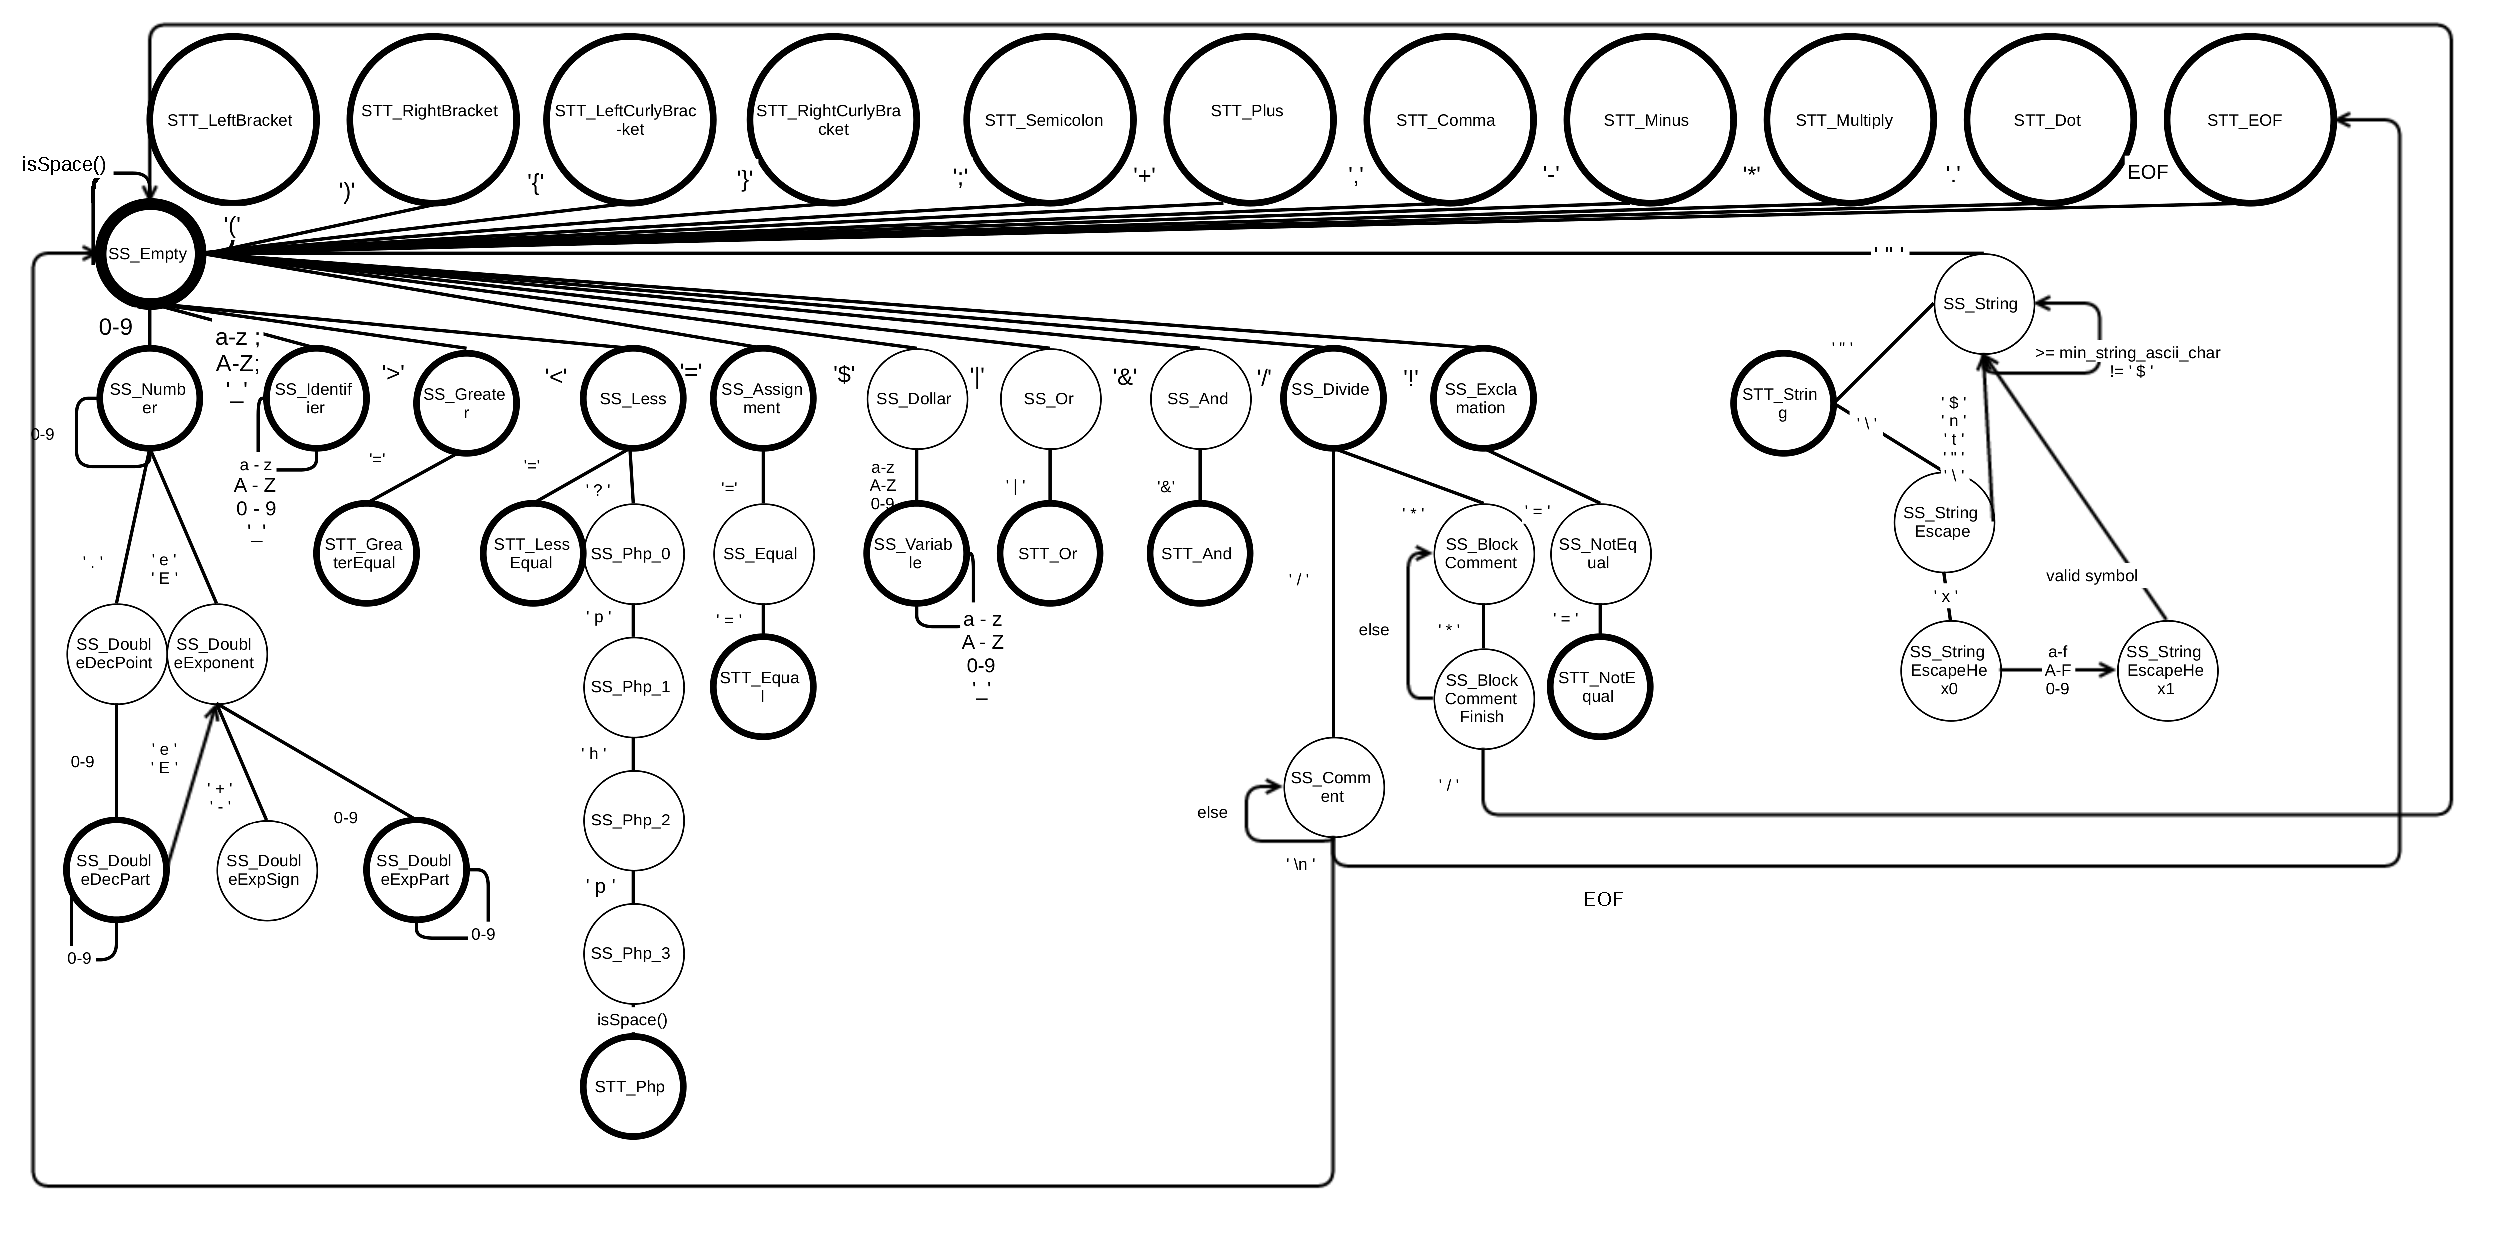
\includegraphics[height=310px]{doc/img/lex_analyza.eps}
\end{sideways}
\end{figure}
\newpage
%=============================================================================
\section{LL gramatika}
1. \textit{PROG} $\rightarrow$ \texttt{<?php} \textit{BODY}\\
2. \textit{BODY} $\rightarrow$ \textit{STMT BODY}\\
3. \textit{BODY} $\rightarrow$ \textit{FUNC BODY}\\
4. \textit{BODY} $\rightarrow$ \texttt{\$}\\
5. \textit{FUNC} $\rightarrow$ \texttt{function id (} \textit{PARAM\_LIST} \texttt{)} \ttlcb  \textit{STMT\_LIST} \ttrcb \\
6. \textit{STMT\_LIST} $\rightarrow$ $\varepsilon$\\
7. \textit{STMT\_LIST} $\rightarrow$ \textit{STMT STMT\_LIST}\\
8. \textit{STMT} $\rightarrow$ \texttt{var\_id =} \textit{EXPR} \ttsc\\
9. \textit{STMT} $\rightarrow$ \texttt{return} \textit{EXPR} \ttsc\\
10. \textit{STMT} $\rightarrow$ \texttt{break} \ttsc\\
11. \textit{STMT} $\rightarrow$ \texttt{continue} \ttsc\\
12. \textit{STMT} $\rightarrow$ \texttt{if (} \textit{EXPR} \texttt{)} \ttlcb \textit{STMT\_LIST} \ttrcb \textit{ELSEIF\_STMT ELSE\_STMT}\\
13. \textit{STMT} $\rightarrow$ \texttt{while (} \textit{EXPR} \texttt{)} \ttlcb \textit{STMT\_LIST} \ttrcb\\
14. \textit{STMT} $\rightarrow$ \texttt{for (} \textit{FOR\_STMT\_1} \ttsc \textit{FOR\_STMT\_2} \ttsc \textit{FOR\_STMT\_1} \texttt{)} \ttlcb \textit{STMT\_LIST} \ttrcb\\
15. \textit{ELSEIF\_STMT} $\rightarrow$ $\varepsilon$\\
16. \textit{ELSEIF\_STMT} $\rightarrow$ \texttt{elseif (} \textit{EXPR} \texttt{)} \ttlcb \textit{STMT\_LIST} \ttrcb \textit{ELSEIF\_STMT}\\
17. \textit{ELSE\_STMT} $\rightarrow$ $\varepsilon$\\
18. \textit{ELSE\_STMT} $\rightarrow$ \texttt{else} \ttlcb \textit{STMT\_LIST} \ttrcb\\
19. \textit{PARAM\_LIST} $\rightarrow$ $\varepsilon$\\
20. \textit{PARAM\_LIST} $\rightarrow$ \texttt{var\_id} \textit{DEF\_ARG NPARAM\_LIST}\\
21. \textit{NPARAM\_LIST} $\rightarrow$ $\varepsilon$\\
22. \textit{NPARAM\_LIST} $\rightarrow$ \texttt{, var\_id} \textit{DEF\_ARG NPARAM\_LIST}\\
23. \textit{DEF\_ARG} $\rightarrow$ $\varepsilon$\\
24. \textit{DEF\_ARG} $\rightarrow$ \texttt{= literal}\\
25. \textit{FOR\_STMT\_1} $\rightarrow$ $\varepsilon$\\
26. \textit{FOR\_STMT\_1} $\rightarrow$ \texttt{var\_id =} \textit{EXPR}\\
27. \textit{FOR\_STMT\_2} $\rightarrow$ $\varepsilon$\\
28. \textit{FOR\_STMT\_2} $\rightarrow$ \textit{EXPR}\\
\newpage
\section{Gramatika pre výrazy}
 \textit{EXPR} $\rightarrow$ \textit{EXPR} \texttt{+} \textit{EXPR} \\
 \textit{EXPR} $\rightarrow$ \textit{EXPR} \texttt{*} \textit{EXPR} \\
 \textit{EXPR} $\rightarrow$ \textit{EXPR} \texttt{-} \textit{EXPR} \\
 \textit{EXPR} $\rightarrow$ \textit{EXPR} \texttt{/} \textit{EXPR} \\
 \textit{EXPR} $\rightarrow$ \textit{EXPR} \texttt{.} \textit{EXPR} \\
 \textit{EXPR} $\rightarrow$ \textit{EXPR} \texttt{<} \textit{EXPR} \\
 \textit{EXPR} $\rightarrow$ \textit{EXPR} \texttt{>} \textit{EXPR} \\
 \textit{EXPR} $\rightarrow$ \textit{EXPR} \texttt{<=} \textit{EXPR} \\
 \textit{EXPR} $\rightarrow$ \textit{EXPR} \texttt{>=} \textit{EXPR} \\
 \textit{EXPR} $\rightarrow$ \textit{EXPR} \texttt{===} \textit{EXPR} \\
 \textit{EXPR} $\rightarrow$ \textit{EXPR} \texttt{!==} \textit{EXPR} \\
 \textit{EXPR} $\rightarrow$ \textit{EXPR} \texttt{\&\&} \textit{EXPR} \\
 \textit{EXPR} $\rightarrow$ \textit{EXPR} \texttt{$\|$} \textit{EXPR} \\
 \textit{EXPR} $\rightarrow$ \textit{EXPR} \texttt{and} \textit{EXPR} \\
 \textit{EXPR} $\rightarrow$ \textit{EXPR} \texttt{or} \textit{EXPR} \\
 \textit{EXPR} $\rightarrow$ \texttt{!} \textit{EXPR} \\
 \textit{EXPR} $\rightarrow$ \texttt{(} \textit{EXPR} \texttt{)} \\
 \textit{EXPR} $\rightarrow$ \texttt{id ( )} \\
 \textit{EXPR} $\rightarrow$ \texttt{id (} \textit{EXPR} \texttt{)}  \\
 \textit{EXPR} $\rightarrow$ \texttt{id (} \textit{EXPR} \texttt{,} \textit{EXPR} \texttt{)} \\
 \textit{EXPR} $\rightarrow$ \texttt{id (} \textit{EXPR} \texttt{,} \textit{EXPR} \texttt{,} \textit{EXPR} \texttt{)} \\
 \textit{EXPR} $\rightarrow$ \texttt{literal} \\
\newpage

%=============================================================================

    \clearpage% Flush earlier floats (otherwise order might not be correct)
    \thispagestyle{empty}% empty page style (?)
    \begin{landscape}% Landscape page
\begin{table}
    \begin{small}
    \begin{tabular}{|c|c|c|c|c|c|c|c|c|c|c|c|c|} \hline
    ~        & {\scriptsize PROG \par} & {\scriptsize BODY \par} & {\scriptsize FUNC \par} & {\scriptsize STMT\_LIST \par} & {\scriptsize STMT \par} & {\scriptsize ELSEIF\_STMT \par} & {\scriptsize ELSE\_STMT \par} & {\scriptsize PARAM\_LIST \par} & {\scriptsize NPARAM\_LIST \par} & {\scriptsize DEF\_ARG \par} & {\scriptsize FOR\_STMT1 \par} & {\scriptsize FOR\_STMT2 \par} \\ \hline
    =        & ~    & ~    & ~    & ~         & ~    & ~           & ~         & ~          & ~           & 24      & ~         & ~         \\ \hline
    var\_id  & ~    & 2    & ~    & 7         & 8    & 15          & 17        & 20         & ~           & ~       & 26        & ~         \\ \hline
    literal  & ~    & ~    & ~    & ~         & ~    & ~           & ~         & ~          & ~           & ~       & ~         & ~         \\ \hline
    ,        & ~    & ~    & ~    & ~         & ~    & ~           & ~         & ~          & 22          & 23      & ~         & ~         \\ \hline
    \}       & ~    & ~    & ~    & 6         & ~    & 15          & 17        & ~          & ~           & ~       & ~         & ~         \\ \hline
    \{       & ~    & ~    & ~    & ~         & ~    & ~           & ~         & ~          & ~           & ~       & ~         & ~         \\ \hline
    else     & ~    & ~    & ~    & ~         & ~    & 15          & 18        & ~          & ~           & ~       & ~         & ~         \\ \hline
    )        & ~    & ~    & ~    & ~         & ~    & ~           & ~         & 19         & 21          & 23      & 25        & ~         \\ \hline
    (        & ~    & ~    & ~    & ~         & ~    & ~           & ~         & ~          & ~           & ~       & ~         & ~         \\ \hline
    elseif   & ~    & ~    & ~    & ~         & ~    & 16          & ~         & ~          & ~           & ~       & ~         & ~         \\ \hline
    ;        & ~    & ~    & ~    & ~         & ~    & ~           & ~         & ~          & ~           & ~       & 25        & 27        \\ \hline
    for      & ~    & 2    & ~    & 7         & 14   & 15          & 17        & ~          & ~           & ~       & ~         & ~         \\ \hline
    while    & ~    & 2    & ~    & 7         & 13   & 15          & 17        & ~          & ~           & ~       & ~         & ~         \\ \hline
    if       & ~    & 2    & ~    & 7         & 12   & 15          & 17        & ~          & ~           & ~       & ~         & ~         \\ \hline
    continue & ~    & 2    & ~    & 7         & 11   & 15          & 17        & ~          & ~           & ~       & ~         & ~         \\ \hline
    break    & ~    & 2    & ~    & 7         & 10   & 15          & 17        & ~          & ~           & ~       & ~         & ~         \\ \hline
    return   & ~    & 2    & ~    & 7         & 9    & 15          & 17        & ~          & ~           & ~       & ~         & ~         \\ \hline
    id       & ~    & ~    & ~    & ~         & ~    & ~           & ~         & ~          & ~           & ~       & ~         & ~         \\ \hline
    function & ~    & 3    & 5    & ~         & ~    & 15          & 17        & ~          & ~           & ~       & ~         & ~         \\ \hline
    \$       & ~    & 4    & ~    & ~         & ~    & 15          & 17        & ~          & ~           & ~       & ~         & ~         \\ \hline
    $\textless$?php      & 1    & ~    & ~    & ~         & ~    & ~           & ~         & ~          & ~           & ~       & ~         & ~         \\ \hline
    \end{tabular}
    \end{small}
    \captionof{table}{LL Tabuľka}
\end{table}
    \end{landscape}
    \clearpage% Flush page
\newpage

%=============================================================================
\section{Inštrukčná sada}

\texttt{IST\_Mov a b}\\
Skopírovanie položky na relatívnej pozícií \texttt{a} do položky na relatívnej pozícií \texttt{b} v aktuálnom zásobnikovom rámci. \\
\\\texttt{IST\_MovC a b} \\
Skopírovanie konštanty v tabuľke konštánt na pozícií \texttt{a} do položky na relatívnej pozícií \texttt{b} v aktuálnom zásobnikovom rámci. \\
\\\texttt{IST\_Jmp dist}\\
Inštrukcia pre vykonanie nepodmieneného skoku.\\
Pripočítanie vzdialenosti(\texttt{dist}) skoku k aktuálnej hodnote \texttt{instruction pointer}u.\\
\\\texttt{IST\_Jmpz dist cond}\\
Inštrukcia pre vykonanie podmieneného skoku.\\
V prípade, že hodnota v operande \texttt{cond} je rovná \texttt{0} tak sa prevedie
pripočítanie vzdialenosti (\texttt{dist}) skoku k aktuálnej hodnote instruction
pointeru.Prevádza sa pretypovanie v prípade nutnosti.\\
\\\texttt{IST\_Jmpnz dist cond}\\
Inštrukcia pre vykonanie podmieneného skoku.\\
V prípade, že hodnota v operande \texttt{cond} nieje rovná '0' tak sa prevedie
pripočítanie vzdialenosti (\texttt{dist}) skoku k aktuálnej hodnote \texttt{instruction pointer}u. \\
\\\texttt{IST\_Push a}\\
Vloženie položky na relatívnej pozícií \texttt{a} na vrchol zásobniku.\\
V prípade, že je položka na relatívnej pozícií typu \texttt{VT\_String}, dôjde k vytvorenie \texttt{Weak Reference}.\\
\\\texttt{IST\_PushC a}\\
Vloženie konštanty na pozícií \texttt{a} v tabuľke konštánt na vrchol zásobniku.\\
\\\texttt{IST\_PushRef a}\\
Na vrchol zásobníku sa vloží \texttt{Strong Reference} na položku na relatívnej pozícií \texttt{a}.\\
Pokiaľ sa na relatívnej pozícií \texttt{a} nachádza \texttt{Strong Reference}, je k jeho hodnote pripočítané \texttt{a}.\\
\\\texttt{IST\_Reserve N}\\
Rezervuje miesto pre \texttt{N} položiek na zásobníku, pre neskoršie použitie.\\
\\\texttt{IST\_Pop N}\\
Zmazanie \texttt{N} položiek z vrcholu zásobníku.\\
\\\texttt{IST\_ClearExpr offset} \\
Vyčistenie zásobníku po vyhodnotení výrazu. V \texttt{offset} je zapísaná pozícia začiatku zásobníkového rámca pre výrazy.\\
\\\texttt{IST\_Call adressIndex}\\
Inštrukcia v vloží na zásobník \texttt{stack pointer} a \texttt{instruction pointer}. Nastaví
\texttt{stack pointer} na miesto kam vložila starý \texttt{stack pointer} a nastaví \texttt{instruction pointer} na adresu
\texttt{AdressTable[adressIndex]}.\\
\\\texttt{IST\_Nullify offset}\\
Nastaví položku na relatívnej pozícií \texttt{offset} v zásobniku na NULL.\\
\\\texttt{IST\_Return a } \\
Zničí aktuálny zásobníkový rámec, pričom načíta starý \texttt{stack pointer} a \texttt{instruction pointer} zo zásobníka.\\
\\\texttt{IST\_BoolVal a res } \\
Prevedie položku na zásobníku na relatívnej adrese \texttt{a} na boolean a výsledok uloží do položky na relatívnej adrese \texttt{res}.\\
\\\texttt{IST\_DoubleVal a res } \\
Prevedie položku na zásobníku na relatívnej adrese \texttt{a} na desatinné číslo a výsledok uloží do položky na relatívnej adrese \texttt{res}.\\
\\\texttt{IST\_IntVal a res } \\
Prevedie položku na zásobníku na relatívnej adrese \texttt{a} na celé číslo a výsledok uloží do položky na relatívnej adrese \texttt{res}.\\
\\\texttt{IST\_StrVal a res } \\
Prevedie položku na zásobníku na relatívnej adrese \texttt{a} na reťazec a výsledok uloží do položky na relatívnej adrese \texttt{res}.\\
\\\texttt{IST\_FindString a b res} \\
Vyhľadá v reťazci \texttt{a} reťazec \texttt{b} a v prípade zhody
uloží index začiatku podreťazca do \texttt{res}.\\
\\\texttt{IST\_GetString res} \\
Načíta reťazec zo štandartného vstupu a uloží do \texttt{res}. \\
\\\texttt{IST\_GetSubString a b res}\\
Vrati podreťazec reťazca, \texttt{a} je začiatočný index a \texttt{b} je
ukončovací index reťazca. Výsledný podreťazec sa bude nachádzať v \texttt{res}.\\
\\\texttt{IST\_PutString res}\\
Vypíše na štandartný výstup reťazec uložený v \texttt{res}.\\
\\\texttt{IST\_SortString a res}\\
Utriedi reťazec uložený v \texttt{res}, \texttt{a} je dĺžka reťazca.\\
\\\texttt{IST\_Add res a b}\\
Vykoná \texttt{a} + \texttt{b} a výsledok uloží do \texttt{res}.\\
\texttt{a}, \texttt{b}, \texttt{res} sú relatívne adresy na základe inštrukčného módu.\\
\\\texttt{IST\_Subtract res a b}\\
Vykoná \texttt{a} - \texttt{b} a výsledok uloží do \texttt{res}.\\
\texttt{a}, \texttt{b}, \texttt{res} sú relatívne adresy na základe inštrukčného módu.\\
\\\texttt{IST\_Multiply res a b}\\
Vykoná \texttt{a} * \texttt{b} a výsledok uloží do \texttt{res}.\\
\texttt{a}, \texttt{b}, \texttt{res} sú relatívne adresy na základe inštrukčného módu.\\
\\\texttt{IST\_Divide res a b}\\
Vykoná \texttt{a} / \texttt{b} a výsledok uloží do \texttt{res}.\\
\texttt{a}, \texttt{b}, \texttt{res} sú relatívne adresy na základe inštrukčného módu.\\
\\\texttt{IST\_Concat res a b}\\
Vykoná konkatenáciu operandov \texttt{a} a \texttt{b} a výsledok uloží do \texttt{res}.\\
\texttt{a}, \texttt{b}, \texttt{res} sú relatívne adresy na základe inštrukčného módu.\\
\\\texttt{IST\_Equal res a b}\\
Porovná či \texttt{a} a \texttt{b} sú rovnakého typu a ak je \texttt{a} rovné \texttt{b}, tak do \texttt{res} vloží \texttt{1}, inak \texttt{0}.\\
\\\texttt{IST\_NotEqual res a b}\\
Porovná či \texttt{a} a \texttt{b} sú rovnakého typu a ak nie je \texttt{a} rovné \texttt{b}, tak do \texttt{res} vloží \texttt{1}, inak \texttt{0}.\\
\\\texttt{IST\_Less res a b}\\
Porovná či \texttt{a} a \texttt{b} sú rovnakého typu a ak je \texttt{a} menšie ako \texttt{b}, tak do \texttt{res} vloží \texttt{1}, inak \texttt{0}.\\
\texttt{a}, \texttt{b}, \texttt{res} sú relatívne adresy na základe inštrukčného módu.\\
\\\texttt{IST\_LessEq res a b}\\
Porovná či \texttt{a} a \texttt{b} sú rovnakého typu a ak je \texttt{a} menšie alebo rovné ako \texttt{b}, tak do \texttt{res} vloží \texttt{1}, inak \texttt{0}.\\
\texttt{a}, \texttt{b}, \texttt{res} sú relatívne adresy na základe inštrukčného módu.\\
\\\texttt{IST\_Greater res a b}\\
Porovná či \texttt{a} a \texttt{b} sú rovnakého typu a ak je \texttt{a} väčšie ako \texttt{b}, tak do \texttt{res} vloží \texttt{1}, inak \texttt{0}.\\
\texttt{a}, \texttt{b}, \texttt{res} sú relatívne adresy na základe inštrukčného módu.\\
\\\texttt{IST\_GreaterEq res a b}\\
Porovná či \texttt{a} a \texttt{b} sú rovnakého typu a ak je \texttt{a} väčšie alebo rovné ako \texttt{b}, tak do \texttt{res} vloží \texttt{1}, inak \texttt{0}.\\
\texttt{a}, \texttt{b}, \texttt{res} sú relatívne adresy na základe inštrukčného módu.\\
\\\texttt{IST\_And a b res}\\
Inštrukcia vykoná logický AND u \texttt{a}, \texttt{b} a výsledok zapíše do \texttt{res}.\\
\texttt{a}, \texttt{b}, \texttt{res} sú relatívne adresy na základe inštrukčného módu.\\
\\\texttt{IST\_Or a b res}\\
Inštrukcia vykoná logický OR u \texttt{a}, \texttt{b} a výsledok zapíše do \texttt{res}.\\
\texttt{a}, \texttt{b}, \texttt{res} sú relatívne adresy na základe inštrukčného módu.\\
\\\texttt{IST\_Not a b res}\\
Inštrukcia vykoná negáciu operandu \texttt{a} ak je operand \texttt{b} rovný \texttt{1}, ak je operand \texttt{b} rovný \texttt{0}
vykoná sa iba konverzia operandu \texttt{a} na údajový typ boolean.\\
% koniec dokumentace
\end{document}
%%%%%%%%%%%%%%%%%%%%%%%%%%%%%%%%%%%%%%%%%%%%%%%%%%%%%%%%%%%%%%%%%%%%%%%%%%%%%%%
